%%%%%%%%%%%%%%%%%%%%%%%%%%%%%%%%%%%%%%%%%%%%%%%%%%%%
%%%% En-tête leçon
\begin{headerBlock}
  \chapter{Interférométrie à division d'amplitude}    \label{LP_DivisionAmplitude}
\end{headerBlock}



%%%%%%%%%%%%%%%%%%%%%%%%%%%%%%%%%%%%%%%%%%%%%%%%%%%%
%%%% Références
\begin{center}
\begin{tabularx}{\textwidth}{| X | X | c | c |}
  \hline
  \rowcolor{gray!20}\multicolumn{4}{c}{Bibliographie de la leçon : } \\
  \hline 
  Titre & Auteurs & Editeur (année) & ISBN \\
  \hline
   Optique physique et électronique  & Daniel Mauras & Presse Universitaire de France (2004) &  \\
  \hline 
   Optique Physique & Richard Taillet & de boeck (2015) & 953-087864-7\\
  \hline 
   Optique & Sylvain Houard & de boeck (2014) & \\
  \hline 
  Optique et phyique ondulatoire & Bertin Faroux Renault & Dunod (1986) & \\
  \hline
\end{tabularx}
\end{center}


%%%%%%%%%%%%%%%%%%%%%%%%%%%%%%%%%%%%%%%%%%%%%%%%%%%%
%%%% Plan
\begin{reportBlock}{Plan détaillé}
  \textbf{Niveau choisi pour la leçon :} Licence 3
  \newline
  \textbf{Prérequis :} Optique Géométrique, Interférences à deux ondes, Interférences à division du front d'onde, cohérence temporelle/cohérence spatiale
  \newline
  
  \textbf{Déroulé détaillé de la leçon: }\newline
  \section*{Introduction : interférences à division du front d'onde}
  Interférences sont beaucoup utilisées en physique et même dans la vie de tous les jours : exemple du casque anti-bruit qui fait interférer les ondes sonores de l'extérieur avec celles du son dans le casque audio.\\
  Dans la suite, on s'intéresse aux interférences à deux ondes lumineuses.\\
  Retour sur les fentes d'Young (\textcolor{green}{slide 1}). Avec un éclairement des fentes par une source ponctuelle, on observe des franges d'interférences non localisées sur un écran.\\
  \textbf{Problème :} (\textcolor{green}{slide 2}) quand on augmente la taille de la source, on observe un brouillage de la figure d'interférences et donc une perte de contraste : problème de cohérence spatiale de la source.\\
  On va voir que l'interférométrie à division d'amplitude permet de s'affranchir de se problème.
  Annonce du plan : 
  \begin{itemize}
      \item Division d'amplitude
      \item Un exemple d'interféromètre à division d'amplitude
      \item Une application pratique de la division d'amplitude
  \end{itemize}
  
  \section{Division d'amplitude}
  \subsection{Théorème de localisation}
  Considérons un système interféromètrique éclairé par une source monochromatique étendue tel que représenté sur la Figure \ref{fig:localisation}. On souhaite qu'au point M, les intensités lumineuses provenant de S et S' qui s'ajoutent ne produisent pas de brouillage. Autrement dit, nous avons la condition de non-brouillage au point M suivante :\newline
  \textcolor{red}{Condition de non-brouillage :} $\Delta(M)=\delta(S',M)-\delta(S,M)=0$ \newline
  On montre (dans D. Mauras p. 159) que :
  \begin{equation}
      -n(\mathbf{u}_2-\mathbf{u}_1)\cdot\mathbf{SS'}=0
  \end{equation}
  Cette équation nous permet de distinguer deux cas :
  \begin{itemize}
      \item $\mathbf{u}_2\ne\mathbf{u}_1$ : c'est une contrainte sur la source, les rayons qui interfèrent en M ne sont pas issus du même rayon incident. C'est le cas des interféromètres à \textbf{division du front d'onde}.
      \item $\mathbf{u}_2=\mathbf{u}_1$ : c'est une contrainte sur l'interféromètre. Les rayons qui interfèrent sont issus du même rayon incident. Le système optique doit contenir une lame séparatrice qui divise en deux un rayon incident puis fait interférer les deux rayons ainsi créés: c'est \textbf{la division d'amplitude}.
  \end{itemize}
  \textcolor{red}{Théorème de localisation :} (\textcolor{green}{Slide 3}) Seuls les dispositifs à division d'amplitude peuvent donner des interférences contrastées produites par des sources arbitrairement larges. Ces interférences sont alors \textbf{localisées} au voisinage des points d'intersection des couples de rayons lumineux issus du même rayon incident.
  
  \subsection{Lame d'air}
  Un exemple simple d'interféromètre à division d'amplitude est celui de la lame d'air. On peut montrer que la différence de marche entre deux rayons lumineux sortant de la lame d'air est donné par :
  \begin{equation}
      \delta(M) = 2ne\cos{i}
  \end{equation}
  avec $e$ l'épaisseur de la lame d'air et $i$ l'angle d'incidence du rayon lumineux provenant de la source S.
  On peut faire quelques remarques : 
  \begin{itemize}
      \item Les interférences sont localisées à l'infini, il faut donc une lentille convergente et un écran placé dans le plan focal image de cette dernière pour observer la figure d'interférences,
      \item Pour une même épaisseur $e$, l'intensité lumineuse ne dépend que de $i$ : on observe des franges circulaires dites \textbf{d'égales inclinaison} qu'on comprend bien en analysant les hyperboloïdes d'interférences (\textcolor{green}{slide 4}),
      \item Pour une source étendue, les franges sont plus brillantes.
  \end{itemize}
  On va voir à présent un système interférométrique réalisant effectivement la lame d'air : il s'agit de l'interféromètre de Michelson.
  
  \section{Interféromètre de Michelson}
  Rappel historique : Expérience de Michelson et Morlay au 19$^{e}$ qui démontre que la vitesse de la lumière est la même dans toutes les directions. Prix Nobel de Physique décerné à Albert Michelson en 1907.
  \subsection{Présentation du montage en configuration lame d'air}
  Le schéma de principe est présenté (\textcolor{green}{slide 5}). Schéma équivalent au tableau tel que représenté sur la Figure \ref{fig:Michelson}.
  Le Michelson n'est certes pas sensible à la cohérence spatiale de la source mais est sensible à sa cohérence temporelle : $\delta(M)\sim 2e<L_c=c\tau_c=c/\Delta\nu=\Delta\lambda/\lambda^2 $. En odg : 
  \begin{itemize}
      \item laser He-Ne à $\Delta\nu=10MHz$, $L_c\sim 30$m
      \item lumière blanche, $L_c\sim 1\mu$m
  \end{itemize}
  Ainsi pour régler le Michelson, on commence par utiliser un laser qui est une source spatialement et temporellement cohérente. Si on souhaite changer de source temporellement moins cohérente que le laser, on se met au contact optique ($e=0$) en utlisant a propriété suivante :on peut montrer que le rayon des anneaux est proportionnel à $1/\sqrt{e}$, ainsi si $e$ diminue, les anneaux s'aggrandissent et rentrent vers leur centre.\newline
  $\rightarrow$ \textcolor{blue}{observation de la figure d'interférence d'un Michelson éclairé par lampe à vapeur de sodium. On voit les anneaux avec une lentille de $f'=20$cm (faible luminosité de la source et salle assez éclairée, utiliser un condenseur à la sortie de la source pour maximiser l'éclairement sur les miroirs) et on peut repérer le contact optique. On observe également un brouillage des franges pour certaines positions du miroir (M1) car doublet du sodium.}\newline
  On va mesurer l'écart en longueur d'onde de ce doublet.
  
  \subsection{Mesure interféromètrique du doublet du sodium}
  On rappelle la formule de l'éclairement pour deux sources lumineuses de longueur d'onde différente (\textcolor{green}{slide 6}). L'écart $\Delta e$ entre deux anticoïncidences est donné par :
  \begin{equation}
      \Delta e = \frac{\bar{{\lambda}}}{2\Delta\lambda^2}
  \end{equation}
  avec $\Delta\lambda =|\lambda_2-\lambda_1|$ et $\bar{{\lambda}}=\frac{\lambda_1+\lambda_2}{2}$.\newline
  $\rightarrow$ \textcolor{blue}{S'éloigner du contact optique de ma nière à pouvoir visualiser 5 ou 6 anticoïncidences. Mesurer $\Delta e$, déterminer $\Delta\lambda$ avec son incertitude et comparer à la valeur tabulée $\Delta\lambda=0,597$nm (Encyclopedia Brittanica).}\\
  Grâce au Michelson, on est capable de faire des mesures interféromètriques très précises (inférieures au nm !).
  
  \section*{Conclusion}
  Présentation de la tomographie en cohérence optique (\textcolor{green}{Slide 7}). Voir R. Taillet.\\
  Ouverture sur le Fabry-Pérot avec la visualisation des anneaux du doublet du sodium obtenues par Fabry-Pérot (contraste des systèmes d'anneaux de $\lambda_1$ et $\lambda_2$) (\textcolor{green}{Slide 8})
\end{reportBlock}

\clearpage
  \begin{figure}[!htbp]
  \centering
  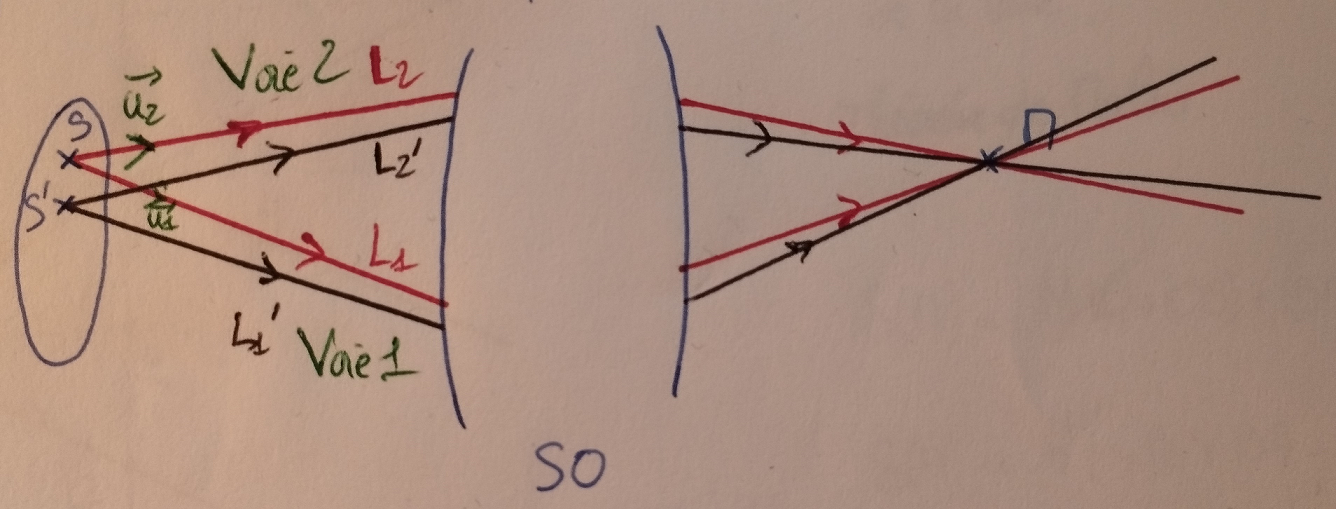
\includegraphics[scale=0.6]{LPO3/localisation.jpg}
  \caption{\label{fig:localisation}Système interférométrique (SO) éclairé par une source étendue. Les voies 1 et 2 constituent les voies de l'interféromètre. S et S' sont deux points sources.}
  \end{figure}
  
  \begin{figure}[!htbp]
  \centering
  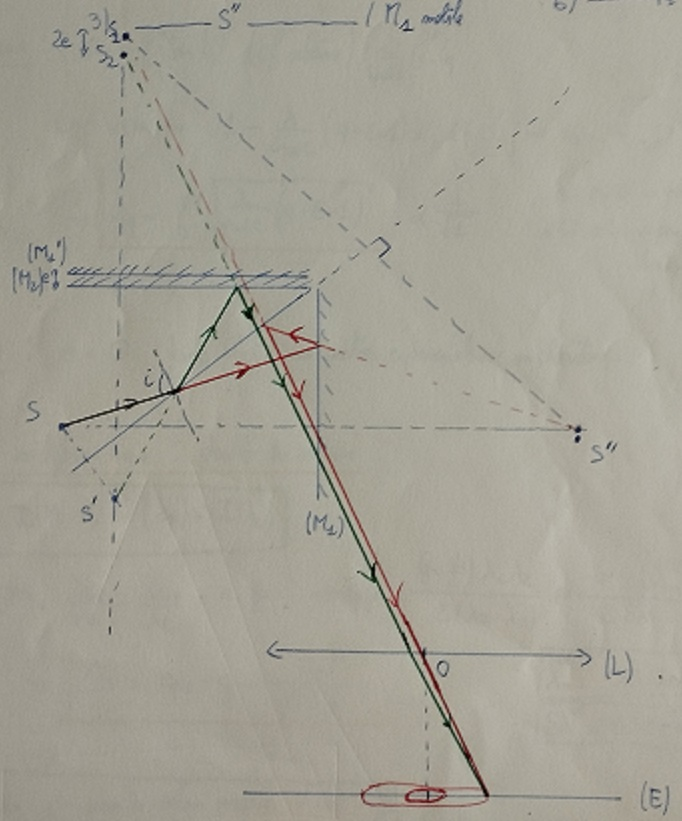
\includegraphics[scale=0.4]{LPO3/Michelson.jpg}
  \caption{\label{fig:Michelson}Schéma équivalent du Michelson. S$_1$ et S$_2$ sont les images de S à travers respectivement la voie 1 (Miroir M1) et la voie 2 (miroir M2) de l'interféromètre. Le miroir (M1') est l'image de (M1) à travers la séparatrice.}
  \end{figure}
  \clearpage
  
  

%%%%%%%%%%%%%%%%%%%%%%%%%%%%%%%%%%%%%%%%%%%%%%%%%%%%
%%%% Questions
\begin{reportBlock}{Questions posées par l’enseignant (avec réponses)}
  \begin{enumerate}
      \item Types d'interférence pour le casque anti-bruit ? \\ \textcolor{purple}{Il y a un micro qui permet d'enregistrer le bruit ambiant. Le signal est ensuite analysé puis un haut-parleur génère un signal de bruit avec une phase exactement opposée à celui qui vient d'être enregistré pour que les deux signaux interfèrent destructivement. Il s'agit donc d'une division du front d'onde.}
      
      \item Utilisation des intérférences à division d'amplitude ? \\
       \textcolor{purple}{Regarder la structure spatiale d'un l'échantillon, voir des défauts de planéité des miroirs, mesurer la différence d'indice de réfraction d'un gaz, mesurer une variation de température}. 
       
    \item Comment mesure-t-on l'indice de réfraction d'un gaz ? \\
       \textcolor{purple}{En configuration lame d'air, on peut regarder comment changent les franges rectlignes lorsque l'indice de refraction $n$ du milieu varie. Connaissant la taille du miroir, on peut remonter à $n$.}
       
      \item Quelle configuration pour la planéité des miroirs ? \\
       \textcolor{purple}{Configuration coin d'air.}
       
      \item En configuration coin d'air, où sont localisées les intérférences ? \\
       \textcolor{purple}{On verra des franges au niveau des miroirs.}
       
     \item Pourquoi au niveau des miroirs ? \\
       \textcolor{purple}{Il faut considérer deux points sources $S_1$ et $S_2$ proches et tracer les rayons issus de ces points et passant par un point $P$. Si $P$ est proches du coin d'air, la différence de marche $\delta_1$ entre les rayons issus de $S_1$ et celle entre les rayons issus de $S_2$ sont quasiment les mêmes (et égales à $2e(P)$): il n'y a donc pas brouillage. En revanche, si $P$ s'éloigne du coin d'air, $\delta_1$ devient très différent de $\delta_2$ et on a brouillage (cf. corrigé du TD d'optique sur les intéreférences). \\
       Par ailleurs, une construction géométrique permet de montrer que le lieu d'intersection des rayons réfléchis correspondant \textbf{à un même rayon incident} (condition de localisation vu en $1.1$, à savoir $\mathbf{u_2} = \mathbf{u_1}$) est approximativement le plan faisant l'angle $i$ (où $i$ est l'angle d'incidence) avec (M1'). En pratique, cet angle est si petit (quelques minutes d'arc) que ce plan d'intersection est presque confondu avec (M1') (Dunod Physique tout-en-un 2ème année, PC-PC* 2004).}
    
    \item Lorsque la source est ponctuelle, les interférences sont-elles localisées ? \\
       \textcolor{purple}{Non. Elles le sont lorsque la source est étendue.}
       
    \item Si on a des trous d'Young et une source déplacée de $b$ sur l'axe parallèle à l'axe des trous, comment seront les franges ? \\
       \textcolor{purple}{Il y aura une différence de chemin optique additionnelle avant les trous. Les nouvelles franges obtenues se décalent de $\frac{-bD}{d}$, avec $d$ la distance entre la source et les trous d'Young et $D$ la distance entre les trous et l'écran.}
    
    \item Peut-il y avoir brouillage si on considère deux sources ponctuelles incohérentes ?\\
    \textcolor{purple}{Oui si les deux systèmes de franges créés par les sources sont en anticoïncidence (les franges brillantes d'un système de franges se superposent aux franges sombres de l'autre système de franges).}
       
    \item Pour la lame d'air, pourquoi appelle-t-on les anneaux "anneaux d'égale inclinaison" ? \\
       \textcolor{purple}{Un ordre d'interférence donné correspond à une inclinaison, c'est-à-dire à un même angle d'incidence des rayons lumineux.}
       
    \item Pour la lame d'air, est-ce qu'on a le même signe de refléxion des deux côtés ? \\
       \textcolor{purple}{Non, $r_1 < 0$, $r_2 > 0$. Il y a un déphasage de $\pi$ en plus. Dans le Michelson, on oublie car c'est plus compliqué que ça, il y a des traitements en plus. Ce qui compte c'est que le contact optique est défini non pas par la longueur géométrique mais par la longueur optique.}
    
    \item A quoi sert la compensatrice ? On pourrait s'en passer pour le laser en réglant la longueur entre les deux bras de sorte à compenser la différence de marche correspondant à l'épaisseur de la séparatrice. \\
       \textcolor{purple}{Si la source est polychromatique, on ne peut pas trouver un pas du miroir qui compense la différence de marche pour toutes les longueurs d'onde car l'indice optique de la séparatrice dépend de la longueur d'onde, d'où la nécessité d'utiliser une compensatrice. Si une seule longueur d'onde, ce n'est pas nécessaire (mais ça n'existe pas dans la vraie vie).}
    
    \item Pourquoi tu utilises un verre anticalorique ? \\
    \textcolor{purple}{Pour ne pas diffuser de la chaleur provenant de la source sur l'interféromètre, cela modifierait $n$ qui dépend de la température (le Michelson est sensible à des variations d'indice de réfraction de l'ordre de $10^{-4}$.)}
       
    \item Le laser He-Ne : 10 MHz. Lorsqu'on a fait le calcul on a trouvé 400 MHz. Pourquoi cette différence ? \\
       \textcolor{purple}{En réalité, le spectre comporte plusieurs raies. L'enveloppe est à 400 MHz mais la largeur de chaque raie est beaucoup moins: 10 MHz semble raisonnable.}

       
    \item Que mesures-tu dans la tomographie ? \\
       \textcolor{purple}{Les interférences associées à une certaine épaisseur.}
      
  \end{enumerate}
\end{reportBlock}


%%%%%%%%%%%%%%%%%%%%%%%%%%%%%%%%%%%%%%%%%%%%%%%%%%%%
%%%% Commentaires
\begin{reportBlock}{Commentaires lors de la correction de la leçon}
\end{reportBlock}


%%%%%%%%%%%%%%%%%%%%%%%%%%%%%%%%%%%%%%%%%%%%%%%%%%%%
%%%% Correction

\begin{reportBlock}{Partie réservée au correcteur}
  \textbf{Avis général sur la leçon (plan, contenu, etc.) :}
  
  
  \textbf{Notions fondamentales à aborder, secondaires, délicates :}
  
  
  \textbf{Expériences possibles (en particulier pour l'agrégation docteur) :}
  
  
  \textbf{Bibliographie conseillée :}
\end{reportBlock}
